%%%%%%%%%%%%%%%%%%%%%%%%%%%%%%%%%%%%%%%%%%%%%%%%%%%%%
%                                                   %
%     Penn State Colloquium Poster Template         %
%                                                   %
% Uses Penn State Colloquium class, with options:   %
%                                                   %
% Orientation:                                      %
%     portrait (default), landscape                 %
%                                                   %
% Paper size:                                       %
%     a4paper (default), a0paper, a1paper, a2paper, %
%     a3paper, a5paper, a6paper                     %
%%%%%%%%%%%%%%%%%%%%%%%%%%%%%%%%%%%%%%%%%%%%%%%%%%%%%
\documentclass{../psuposter}
\renewcommand{\templateimagepath}{../} 


%%%%%%%%%%%%%%%%%%%%%%%%%%%%%%%%%%%%%%%%%%%%%%%%%%%%%
%               Package Dependencies                %
%%%%%%%%%%%%%%%%%%%%%%%%%%%%%%%%%%%%%%%%%%%%%%%%%%%%%
\usepackage{natbib}
\usepackage{lipsum}                                % Dummy text
\usepackage[figwidth = 0.98\linewidth]{todonotes}  % Dummy image (and more!)
\usepackage[absolute, overlay]{textpos}            % Figure placement
\usepackage{braket}
\setlength{\TPHorizModule}{\paperwidth}
\setlength{\TPVertModule}{\paperheight}
\setcitestyle{numbers,square}


%%%%%%%%%%%%%%%%%%%%%%%%%%%%%%%%%%%%%%%%%%%%%%%%%%%%%
%                 AUTHOR AND TITLE                  %
%%%%%%%%%%%%%%%%%%%%%%%%%%%%%%%%%%%%%%%%%%%%%%%%%%%%%
\title{High-Energy Neutrino Astrophysics in the Multimessenger Era}
\author{Kohta Murase}
\institute{Penn State University}


%%%%%%%%%%%%%%%%%%%%%%%%%%%%%%%%%%%%%%%%%%%%%%%%%%%%%
%                  BEGIN DOCUMENT                   %
%%%%%%%%%%%%%%%%%%%%%%%%%%%%%%%%%%%%%%%%%%%%%%%%%%%%%
\begin{document}
\begin{frame}
\begin{columns}[t, totalwidth=\textwidth]
\begin{column}{0.45\textwidth - 1cm}


%%%%%%%%%%%%%%%%%%%%%%%%%%%%%%%%%%%%%%%%%%%%%%%%%%%%%
%                 BLOCK: BIOGRAPHY                  %
%%%%%%%%%%%%%%%%%%%%%%%%%%%%%%%%%%%%%%%%%%%%%%%%%%%%%
    \begin{block}{Speaker Biographic Summary}
    	\begin{center}
    		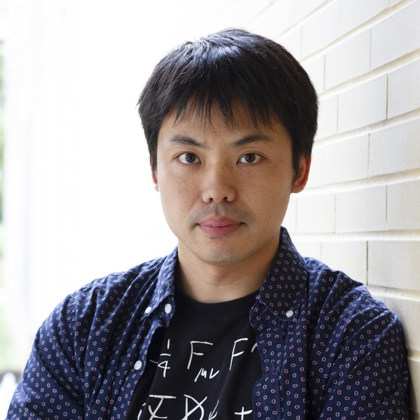
\includegraphics[width=0.6\textwidth]{images/murase}
    	\end{center}
    	\href{https://science.psu.edu/physics/people/kohta-murase}{Dr. Kohta Murase} is an assistant professor of Physics and Astronomy \& Astrophysics at Penn State. Professor Murase joined Penn State as a faculty in 2015 and has been involved in research at the interface of frontiers of theoretical high-energy astrophysics, gravitational, particle and nuclear physics. His research has established new paradigms for experimental observations such as the production of PeV neutrinos. His current research interests are in utilizing recent discoveries by LIGO and multi-messenger astronomy to study the nature of and detect exotic high energy cosmic particles. Professor Murase's honors include the Nishinomiya-Yukawa Memorial Prize (2019), the Alfred P. Sloan Research Fellowship (2017), Young Scientist Award of the Physical Society of Japan (2016), and Young Scientist Award of the Astronomical Society of Japan (2015).
    \end{block}


%%%%%%%%%%%%%%%%%%%%%%%%%%%%%%%%%%%%%%%%%%%%%%%%%%%%%
%            BLOCK: RESEARCH INTERESTS              %
%%%%%%%%%%%%%%%%%%%%%%%%%%%%%%%%%%%%%%%%%%%%%%%%%%%%%
    \begin{block}{Research Interests}
        Prof. Murase's research focuses on astroparticle physics, including neutrinos, gamma rays, cosmic rays, gravitational waves, and dark matter. He is also interested in related high-energy astrophysics, such as the multi-messenger study of extreme astrophysical objects.
        \begin{center}
	    	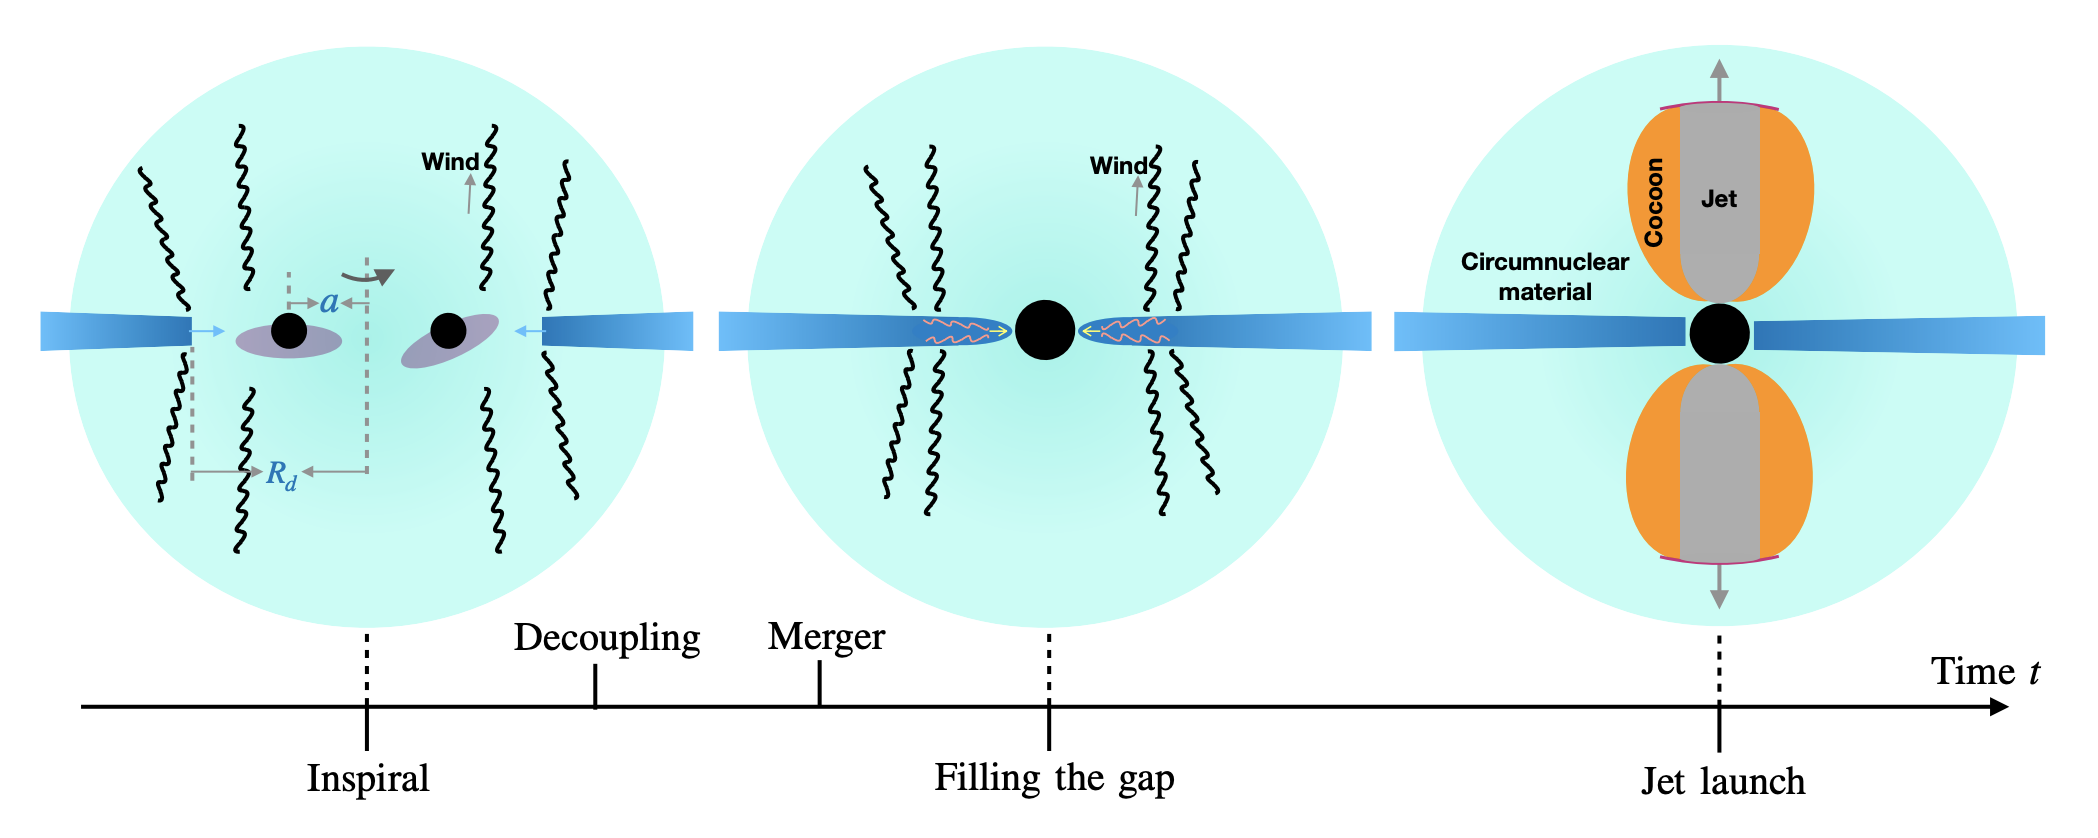
\includegraphics[width=0.95\textwidth]{images/minidisk}    		
    	\end{center}
    	\textit{Schematic of the merger of supermassive black holes with minidisks, including disk wind and jet-cocoon.} \cite{yuanHighenergyNeutrinoEmission2020}
    \end{block}
\end{column}
\begin{column}{0.55\textwidth - 1cm}


%%%%%%%%%%%%%%%%%%%%%%%%%%%%%%%%%%%%%%%%%%%%%%%%%%%%%
%                 BLOCK: ABSTRACT                   %
%%%%%%%%%%%%%%%%%%%%%%%%%%%%%%%%%%%%%%%%%%%%%%%%%%%%%
    \begin{block}{Talk Abstract}
         The discovery of high-energy cosmic neutrinos opened a new window of astroparticle physics. Their origin is a new mystery in the field, which is tightly connected to the long-standing puzzle about the origin of cosmic rays. I will discuss theoretical implications of the latest results on high-energy neutrino and cosmic-ray observations, and demonstrate the power of multi-messenger approaches. In particular, I will show that the observed fluxes of neutrinos, gamma rays, and extragalactic cosmic rays can be understood in a unified manner. I will also highlight our recent developments about astrophysical neutrino emission from gamma-ray dark sources and violent transient phenomena such as supermassive black hole flares. I may discuss some possibilities of utilizing high-energy neutrinos as a probe of physics beyond the Standard Model.
    \end{block}


%%%%%%%%%%%%%%%%%%%%%%%%%%%%%%%%%%%%%%%%%%%%%%%%%%%%%
%                BLOCK: BACKGROUND                  %
%%%%%%%%%%%%%%%%%%%%%%%%%%%%%%%%%%%%%%%%%%%%%%%%%%%%%
    \begin{block}{Brief Background}
        Real-time observations of high-energy (HE) neutrinos have enabled a new era  multi-messenger particle astrophysics. These observations have allowed for the analysis of HE phenomena caused by super-massive black holes (SMBH), as well as the constaint of HE cosmic-ray (CR) acceleration in powerful jets. \cite{muraseHighEnergyNeutrinoGammaRay2020} Tidal disruption events (TDE), which have been suggested as sources of ultrahigh-energy cosmic rays, and recent multi-messenger events have helped investigate neutrino production models in TDE environments.

        \begin{center}
		   	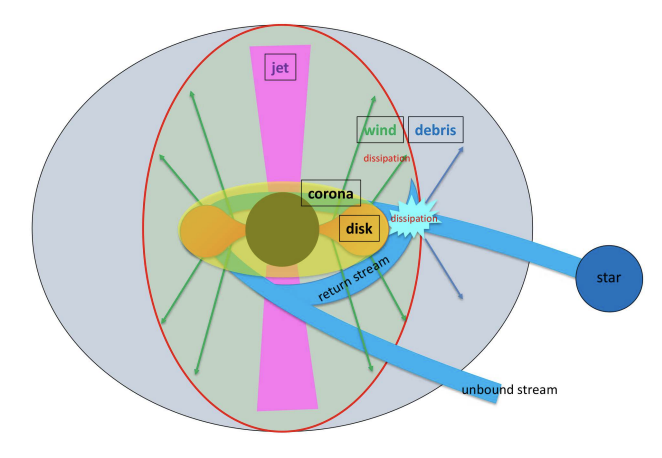
\includegraphics[width=0.65\textwidth]{images/production}    		
    	\end{center}
		 Some TDE neutrino-production models, including core models, hidden-wind models, and jet models, are depicted schematically (above). \cite{muraseHighEnergyNeutrinoGammaRay2020} Core models involve disrupted stellar material falling back and accreting onto the SMBH. Hidden wind models represent the bound stellar material in highly eccentric trajectories around the SMBH, undergoing various dissipative processes. In jet models, the bound stellar material is ejected in relativistic streams. \cite{muraseHighEnergyNeutrinoGammaRay2020}

    \end{block}


%%%%%%%%%%%%%%%%%%%%%%%%%%%%%%%%%%%%%%%%%%%%%%%%%%%%%
%                 BLOCK: REFERENCES                 %
%%%%%%%%%%%%%%%%%%%%%%%%%%%%%%%%%%%%%%%%%%%%%%%%%%%%%
    \begin{block}{References}
        \bibliographystyle{aipnum4-1}
%        \bibliographystyle{iopart-num}
		\bibliography{references}
    \end{block}

\end{column}
\end{columns}


%%%%%%%%%%%%%%%%%%%%%%%%%%%%%%%%%%%%%%%%%%%%%%%%%%%%%
%                    FOOTER TEXT                    %
%%%%%%%%%%%%%%%%%%%%%%%%%%%%%%%%%%%%%%%%%%%%%%%%%%%%%
\begin{textblock}{0.5}(0.18, 0.94)
    \color{white}
    \sffamily
    \textbf{Eberly College of Science}
    \\
    Department of Physics
\end{textblock}


%%%%%%%%%%%%%%%%%%%%%%%%%%%%%%%%%%%%%%%%%%%%%%%%%%%%%
%                   END TEMPLATE                    %
%%%%%%%%%%%%%%%%%%%%%%%%%%%%%%%%%%%%%%%%%%%%%%%%%%%%%
\end{frame}
\end{document}
